\documentclass[a4paper]{article}
\usepackage[spanish]{babel}
\usepackage[utf8]{inputenc}
\usepackage{charter}   % tipografia
\usepackage{graphicx}


%%%%%%%LO AGREGUE%%%%%%%%%%  Y yo lo modifique
%\usepackage{hyperref}
%%%%%%%%%%%%%%%%%%%%%%%%%%

\usepackage[bookmarks = true, colorlinks=true, linkcolor = black, citecolor = black, menucolor = black, urlcolor = blue]{hyperref} 




%\usepackage{makeidx}
\usepackage{paralist} %itemize inline
\usepackage[ruled,vlined]{algorithm2e}
%\usepackage{float}
%\usepackage{amsmath, amsthm, amssymb}
%\usepackage{amsfonts}
%\usepackage{sectsty}
%\usepackage{charter}
%\usepackage{wrapfig}
%\usepackage{listings}
%\lstset{language=C}


\usepackage{color} % para snipets de codigo coloreados
\usepackage{fancybox}  % para el sbox de los snipets de codigo

\definecolor{litegrey}{gray}{0.94}

% \newenvironment{sidebar}{%
% 	\begin{Sbox}\begin{minipage}{.85\textwidth}}%
% 	{\end{minipage}\end{Sbox}%
% 		\begin{center}\setlength{\fboxsep}{6pt}%
% 		\shadowbox{\TheSbox}\end{center}}
% \newenvironment{warning}{%
% 	\begin{Sbox}\begin{minipage}{.85\textwidth}\sffamily\lite\small\RaggedRight}%
% 	{\end{minipage}\end{Sbox}%
% 		\begin{center}\setlength{\fboxsep}{6pt}%
% 		\colorbox{litegrey}{\TheSbox}\end{center}}

\newenvironment{codesnippet}{%
	\begin{Sbox}\begin{minipage}{\textwidth}\sffamily\small}%
	{\end{minipage}\end{Sbox}%
		\begin{center}%
		\vspace{-0.4cm}\colorbox{litegrey}{\TheSbox}\end{center}\vspace{0.3cm}}



\usepackage{fancyhdr}
\pagestyle{fancy}

%\renewcommand{\chaptermark}[1]{\markboth{#1}{}}
\renewcommand{\sectionmark}[1]{\markright{\thesection\ - #1}}

\fancyhf{}

\fancyhead[LO]{Sección \rightmark} % \thesection\ 
\fancyfoot[LO]{\small{Agustina Aldasoro, Francisco Noriega, Ezequiel Zimenspitz, Brian Zuker}}
\fancyfoot[RO]{\thepage}
\renewcommand{\headrulewidth}{0.5pt}
\renewcommand{\footrulewidth}{0.5pt}
\setlength{\hoffset}{-0.8in}
\setlength{\textwidth}{16cm}
%\setlength{\hoffset}{-1.1cm}
%\setlength{\textwidth}{16cm}
\setlength{\headsep}{0.5cm}
\setlength{\textheight}{25cm}
\setlength{\voffset}{-0.7in}
\setlength{\headwidth}{\textwidth}
\setlength{\headheight}{13.1pt}

\renewcommand{\baselinestretch}{1.1}  % line spacing


% \setcounter{secnumdepth}{2}
\usepackage{underscore}
\usepackage{caratula}
%\usepackage{url}
\usepackage{hyperref}

% ******************************************************** %
%              TEMPLATE DE INFORME ORGA2 v0.1              %
% ******************************************************** %
% ******************************************************** %
%                                                          %
% ALGUNOS PAQUETES REQUERIDOS (EN UBUNTU):                 %
% ========================================
%                                                          %
% texlive-latex-base                                       %
% texlive-latex-recommended                                %
% texlive-fonts-recommended                                %
% texlive-latex-extra?                                     %
% texlive-lang-spanish (en ubuntu 13.10)                   %
% texlive-science										  %
% ******************************************************** %



\begin{document}


\thispagestyle{empty}
\materia{Algoritmos y Estructuras de Datos III}
\submateria{Primer Cuatrimestre de 2015}
\titulo{Trabajo Práctico I}
%\subtitulo{subtitulo del trabajo}
\integrante{Aldasoro Agustina}{86/13}{agusaldasoro@gmail.com}
\integrante{Noriega Francisco}{XXX/XX}{mail}
\integrante{Zimenspitz Ezequiel}{155/13}{ezeqzim@gmail.com}
\integrante{Zuker Brian}{XXX/XX}{mail}


\maketitle
\newpage

\thispagestyle{empty}
\vfill
\begin{abstract}
Habi\'endonos sido dado una serie de tres problem\'aticas a resolver, se plantean sus respectivas soluciones acorde a los requisitos pedidos. Se adjunta una descripci\'on de cada problema y su soluci\'on, conjunto a su an\'alisis de correctitud y de complejidad sumado a su experimentaci\'on. El lenguaje elegido para llevar a cabo el trabajo es C++.
\end{abstract}

\thispagestyle{empty}
\vspace{3cm}
\tableofcontents
\newpage


%\normalsize
\newpage

\section{Problema 1: ZombieLand}

\subsection{Descripci\'on de la problem\'atica}

Dado un mapa con \emph{n} ciudades, en cada una de ellas se encuentra una determinada cantidad de Zombies y una determinada cantidad de Soldados (ambas tambi\'en dadas). El objetivo del problema es exterminar a la invasi\'on zombie, para ello es necesario un enfrentamiento \textit{zombies vs soldados} por cada ciudad. Con el fin de que este enfrentamiento sea positivo, es decir se logre matar a todos los zombies de una ciudad, es necesario que la cantidad de zombies sea, a lo sumo, diez veces m\'as grande que la cantidad de soldados.\\

Como los soldados se encuentran atrincherados, se puede optar entre llevar a cabo un enfrentamiento o no (ya que no se desea provocar un ataque donde ya se sabe que se va a perder). Los soldados acuartelados no pueden moverse de la ciudad en la que est\'an, pero s\'i se cuenta con una dotaci\'on de soldados extra que se la puede ubicar en cualquiera de las \emph{n} ciudades acorde a lo deseado. La cantidad de soldados extra es ilimitada, mas los recursos para trasladarlos no lo son. El traslado de cada soldado extra a una ciudad tiene un costo espec\'ifico que var\'ia acorde a la ciudad elegida. Siempre que sea econ\'omicamente posible, se puede trasladar una cantidad de soldados indistinta por ciudad.\\

Debido a que los recursos econ\'omicos son finitos, no siempre va a ser posible salvar a las n ciudades. Lo que se desea en este problema es maximizar la cantidad de ciudades salvadas, respetando el presupuesto. Es decir, se deben establecer las cantidades de soldados extras enviados a cada ciudad de modo que la cantidad de ciudades salvadas sea la \'optima y gastando un monto por debajo del presupuesto.  El algoritmo debe tener una complejidad temporal de $O(n.log(n))$, siendo $n$ la cantidad de ciudades del pa\'is.\\

\textcolor{red}{Aca se podr\'ia poner unos dibujitos de soluciones \'optimas como para que quede m\'as lindo}


\newpage
\subsection{Resoluci\'on propuesta y justificaci\'on}

\textcolor{red}{Ver que habla mucho sobre vectores y dijo que no mezclaramos implementacion con algoritmo}\\

Para la resoluci\'on del problema decidimos utilizar un algoritmo goloso, el mismo tomar\'a una decisi\'on \'optima para cada instante, sin revisar si ser\'a la mejor a nivel global.\\

Como primera instancia, el algoritmo simplemente calcula, para cada ciudad, cu\'anto ser\'ia el costo de salvarla. Para ello, primero se calcula la cantidad de soldados extra necesarios y luego se multiplica por el costo de traslado de cada unidad:\\


	\begin{codesnippet}
	\begin{verbatim}
		soldados_extras_necesarios = redondeo_hacia_arriba((zombies - (soldados_existentes * 10)) /10)
		
		costo_total = costo_unitario * soldados_extras_necesarios
	\end{verbatim}
	\end{codesnippet}

Luego de haber obtenido una magnitud con la cual se pueden comparar las ciudades entre s\'i, se ordenan las ciudades de menor a mayor en base al costo de salvarla para ser recorridas secuencialmente y enviar los ej\'ercitos requeridos hasta que alcance el presupuesto.\\

 Como las ciudades van a estar almacenadas en un vector, en la posicion \textit{vec}$_0$ se va a encontrar la ciudad que es m\'as barata de salvar y en la posici\'on \textit{vec}$_{n-1}$ la m\'as cara. En este vector se van a encontrar todas las ciudades pasadas por par\'ametro, sin importar que una ciudad ya este salvada al ser ingresada.\\
 
 Se recorre este vector secuencialmente, de modo que para cada posici\'on i $\in$ [0,n-1] se va a comparar el costo de salvar la ciudad \emph{i} contra el presupuesto restante en esa instancia (presupuesto_actual). Si es una compra factible, se resta el costo_total del presupuesto_actual y se envian las tropas necesarias a la ciudad \emph{i}; en caso contrario se le asigna \emph{0} a las tropas extras enviadas a la ciudad \emph{i}. \\
 
 Por la forma en que fue construido el vector, cuando se encuentre una ciudad i que el costo de salvarla excede del presupuesto_actual las dem\'as ciudades j $\in$ [i+1, n-1] tampoco podr\'an ser salvadas. De todos modos, nuestro algoritmo realiza el mismo c\'alculo para todas las posiciones del vector.\\
 
Como en este vector las ciudades no aparecen en orden creciente por su n\'umero, debemos reordenarlas. Debido a que el \emph{id} de cada ciudad va a ser \'unico y va a encontrarse en el intervalo [0, n-1], se lo recorre secuencialmente colocando cada ciudad en la posici\'on de su \textit{id} dentro de un nuevo vector \emph{respuesta} . \textcolor{red}{Ver que este parrafo me aprece que no quedo muy claro...} \\
 
 
 

El algortimo resuelve el problema salvando la mayor cantidad de ciudades posibles porque
\textcolor{red}{INSERT FORMAL DEMO}

\newpage
\subsection{An\'alisis de la complejidad}
La complejidad de nuestra soluci\'on es $O(n.log(n))$, siendo \emph{n} la cantidad de ciudades del pa\'is.\\



Como primera instancia, el algoritmo almacena las ciudades con sus caracter\'isticas (pasadas como par\'ametro) dentro de un vector para luego poder utilizarlas de un modo pr\'actico. Como esto lo realiza secuencialmente, tiene un costo lineal \textbf{\textit{O(n)}}. \textcolor{red}{Esto habia que ponerlo aca asi? o directamente nada? o solo nombrarlo?}\\

\begin{algorithm}[h!]
\caption{zombieland}
\For{\emph{cada} ciudad \emph{en vector} pa\'is}{
	Calcular la cantidad de soldados extra necesarios y el costo de esto.\\
	Almacenar esta informaci\'on en un vector \emph{datos} mediante \textit{push_back()}
}
Ordena al vector \emph{datos} mediante \textit{sort_heap()}\\
\For{\emph{cada} ciudad \emph{en vector} datos}{
	Calcular si puede ser salvada.\\
	Indicarle cantidad de soldados extras enviados y cambios en el presupuesto_actual.
}
\For{\emph{cada} ciudad \emph{en vector} datos}{
	Insertar en el vector \emph{respuesta}[ciudad.id] la ciudad actual. 
}
\end{algorithm}
\textcolor{red}{En el codigo, yo pondria este reordenamiento dentro de zombieland, ya que hay que considerarlo para medir tiempos.}\\

El c\'odigo presenta un \textbf{primer ciclo \emph{for}} que calcula el costo de salvar a cada ciudad y las agrega mediante push_back() a un vector. El ciclo recorre linealmente todas las ciudades por lo que tiene complejidad $O(n)$. 

El c\'alculo de salvar a cada ciudad coincide con el descripto en la secci\'on anterior, el cual por ser operaciones aritm\'eticas es $O(1)$. Armar el nuevo struct para insertar dentro del vector \emph{datos} tambi\'en posee un costo constante $O(1)$. La funci\'on \href{http://www.cplusplus.com/reference/vector/vector/push_back/}{push\_back()} \footnote{http://www.cplusplus.com/reference/vector/vector/push_back/} tiene costo $O(1)$ amortizado, lo que implica que cuando no precisa redimensionar el vector cuesta esto, y cuando lo hace, toma tiempo lineal en la cantidad de elementos. Como insertamos durante todo el ciclo tomamos el costo amortizado $O(1)$. 

Por lo tanto, la complejidad total del primer ciclo for nos da \textbf{\textit{O(n)}}.\\

Le sigue \textbf{ordenar el vector} con estos datos, para ello usamos \href{http://www.cplusplus.com/reference/algorithm/sort_heap/?kw=sort_heap}{sort\_heap()} \footnote{http://www.cplusplus.com/reference/algorithm/sort_heap/?kw=sort_heap} de la librer\'ia de \emph{C} cuya complejidad es \textbf{\textit{O(n.log(n)})}.\\

A continuaci\'on, se realiza un \textbf{\'ultimo ciclo \emph{for}} que salva las ciudades que pueda, mientras dure el presupuesto y deja en \emph{0 soldados enviados} a las ciudades que no pueden ser salvadas. Estos c\'alculos aritm\'eticos y asignaciones son todos de complejidad constante O(1). Este ciclo recorre linealmente todas las ciudades por lo tanto, lo hace con complejidad \textbf{\textit{O(n)}}.\\

Finalmente, se debe \textbf{reordenar el vector} obtenido hasta ahora para que quede en orden creciente respecto de su \textit{id}. Como esto se hace recorriendo secuencialmente el primer vector, asign\'andole uno a uno los elementos al nuevo vector \emph{respuesta} indexados; s\'olo hace una pasada lineal con costo \textbf{\textit{O(n)}}.\\



Como cada paso de los mencionados son secuenciales, las complejidades se suman, obteniendo:

 $O(n)$ + $O(n.log(n))$ + $O(n)$ + $O(n)$ que es igual a \textit{\textbf{O(n.log(n))}} por propiedades de $O$.


\newpage

\subsection{C\'odigo fuente}

	\begin{codesnippet}
	\begin{verbatim}
struct ciudad{
    int zombies;
    int soldados;
    int costo;
};
	\end{verbatim}
	\end{codesnippet}

	\begin{codesnippet}
	\begin{verbatim}
struct ciudad2{
    int numCiudad;
    int soldadosNecesarios;
    int costoTotal;
    bool operator< (const ciudad2& otro) const{
        return costoTotal < otro.costoTotal;
    }
};
	\end{verbatim}
	\end{codesnippet}

\textcolor{red}{Poner como leemos y escribimos?? y el main? CREO QUE SI...}


\begin{algorithm}[h!]
\caption{ZombieLand(\textit{out}: vector$<$ciudad2$>$; \textit{in}: int cantCiudades, int presupuesto, vector$<$ciudad$>$\& pais; \textit{in/out}:  int\& salvadas)}
salvadas = 0;\\
vector$<$ciudad2$>$ datos;\\
\For{(int i = 0; i $<$ cantCiudades; ++i)}{
	ciudad2 actual;\\
	actual.numCiudad = i;\\
	double diferencia = (pais[i].zombies - pais[i].soldados * 10);\\
	\eIf{(diferencia $>$ 0)}{
	actual.soldadosNecesarios = ceil(diferencia/10);
	}{
	actual.soldadosNecesarios = 0;
	}
	actual.costoTotal = actual.soldadosNecesarios * pais[i].costo;\\
		datos.push_back(actual);
}
sort_heap(datos.begin(), datos.end());\\
\For{(int i = 0; i $<$ cantCiudades; ++i)}{
	int dif = presupuesto - datos[i].costoTotal;\\
	\eIf{(dif$>=$0)}{salvadas++;\\
			presupuesto = dif;}{datos[i].soldadosNecesarios = 0;}
}
\textbf{return} datos;
\end{algorithm}

\textcolor{red}{No segui poniendo el algoritmo, por si le tenemos que hacer algun cambio.}

\newpage
\subsection{Experimentaci\'on}

\noindent Experimentos que se pueden hacer:

-Muchas ciudades con pocos soldados para mandar, pero presupuesto bajo. Hipotesis: realmente es la cantidad optima, sin importar la que elija.

-Una cantidad muy grande de ciudades y todas salvadas ya al ser ingresadas VS la misma cantidad de ciudades pero ahora hay un presupuesto grande y hay que elegir. Hipotesis: ambas deberian tardar tiempos similares.

-Mejorar el algortimo para que cuadno encuentra uan ciudad que no puede salvar, ya no recorra mas. Y comparar tiempos del ejemplo anterior. Hipotesis: el tiempo en el primer caso deberia ser notoriamente inferior.

-Comparar tiempos para ciudades de tama\~no 10, 100, 1000, 10000 y 100000 generando aleatoriamente diez de cada una y scar promedio.\\



\textcolor{red}{Ver bien como generar ciudades aleatorias}

\newpage

\section{Problema 2: Alta Frecuencia}
\subsection{Descripci\'on de la problem\'atica}

Se quiere transmitir informaci\'on secuencialmente mediante un enlace el mayor tiempo posible. Los enlaces tienen asociadas distintas frecuencias, con un costo por minuto y un intervalo de tiempo (sin cortes) en el cual funcionan. Se utilizan durante minutos enteros, y es posible cambiar de una frecuencia a otra instant\'anemente (del minuto 1 al 4 uso la frecuencia A y del 4 al 6 la B). Los datos del precio y e intervalo de tiempo de cada frecuencia son dados. Se desea optimizar este problema para transmitir todo el tiempo que tenga al menos una frecuencia abierta, pero gastando la menor cantidad de dinero. Se debe contar con una complejidad de $O(n.log(n))$.\\

A continuaci\'on se muestran dos casos particulares de este problema. En ambos se ofrecen tres frecuencias, con distintos costos cada una. Se puede ver recuadrado en violeta cu\'al es la elecci\'on que debe hacerse por intervalo de tiempo.


 \begin{figure}[h!]
   \begin{center}
 	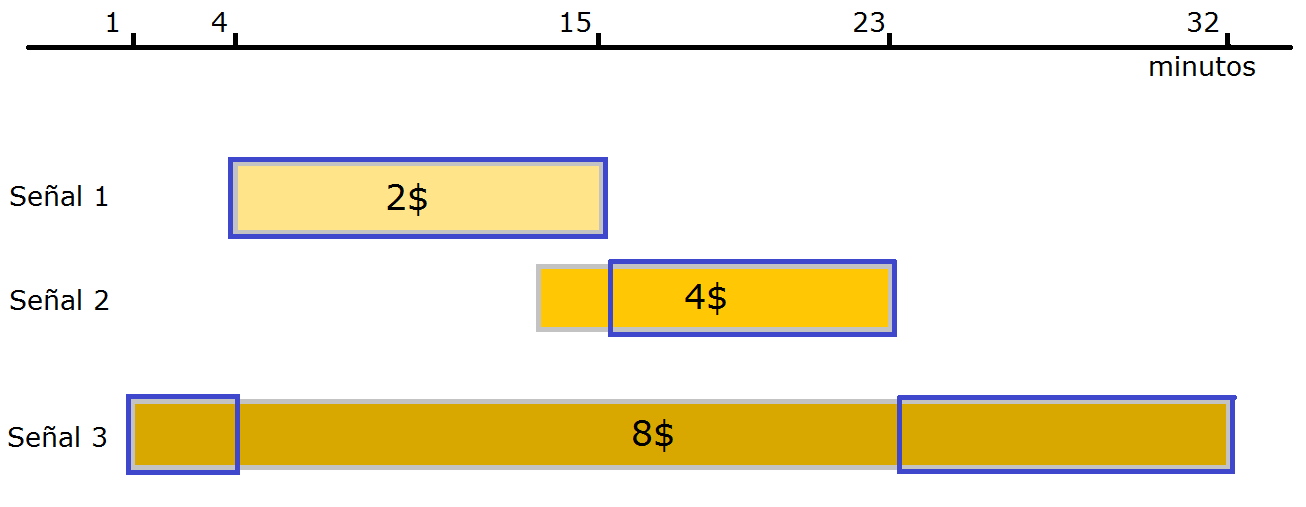
\includegraphics[scale=0.45]{imagenes/ej2/ejemplo1.png}
 	\caption{Ejemplo 1}
% 	\label{caballito}	
   \end{center}
 \end{figure}

 \begin{figure}[h!]
   \begin{center}
 	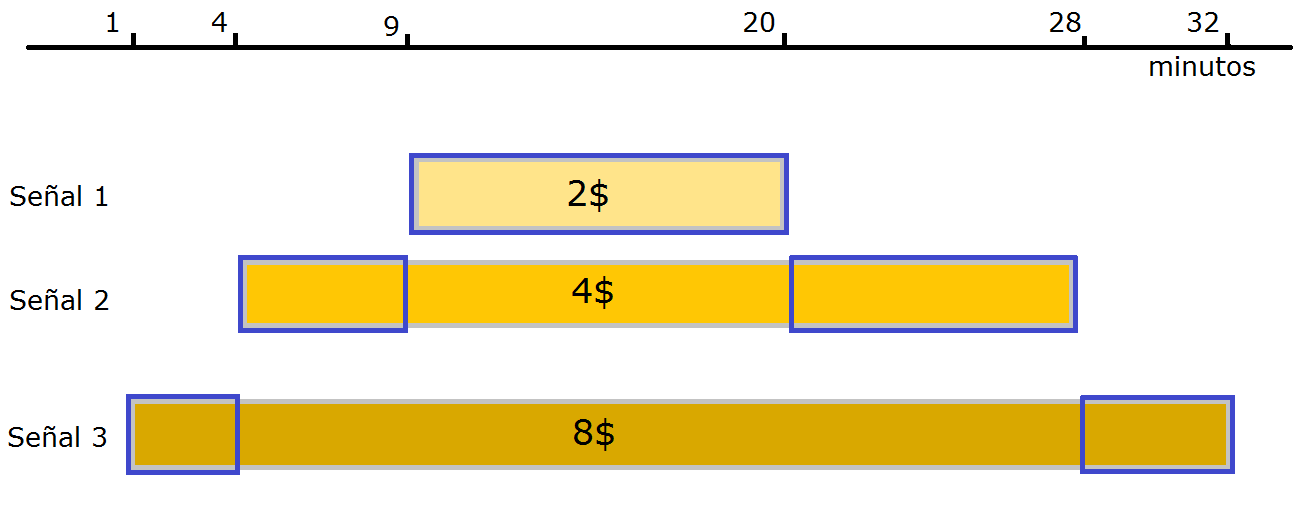
\includegraphics[scale=0.45]{imagenes/ej2/ejemplo2.png}
 	\caption{Ejemplo 1}
% 	\label{caballito}	
   \end{center}
 \end{figure}


\newpage

\subsection{Resoluci\'on propuesta y justificaci\'on}

El algoritmo que utilizamos pertenece a la familia de \emph{Divide \& Conquer}.\\

\textcolor{red}{Aca pasa lo mismo de la implementacion porque hablamos mucho de vector y bla...}\\

Todas las frecuencias se encuentran almacenadas en un vector. Primero se las ordena en orden creciente respecto del costo, es decir en la primera posición se almacena la m\'as barata y en la última, la más cara. Una vez que contamos con este ordenamiento inicial, se va a proseguir mediante el \emph{divide} dentro de este vector.\\

Se prosigue de acuerdo a las características de Divide \& Conquer. De modo recursivo, se divide al vector pasado por parámetro por la mitad creando dos nuevos a los cuales se les aplica nuestro algoritmo de merge. El caso base se da cuando el vector tiene un sólo elemento, para lo cual se devuelve el vector tal cual entró.\\

Nuestro algoritmo de Merge se encarga de elegir entre las frecuencias de dos arreglos pasados como parámetro, de modo que devuelve un sólo vector indicando los intervalos ocupados por las frecuencias elegidas. 

Dado el enunciado del problema, para elegir qu\'e frecuencia utilizar en determinado intervalo de tiempo se debe priorizar el precio más barato emitiendo señal siempre que sea posible. Gracias a que en el primer llamado de nuestra funci\'on estas se encontraban en orden creciente respecto del costo, en cada paso de \emph{merge} de los dos arreglos de entrada con intervalos se van a priorizar los de la izquierda. Es decir que en cada paso, todos los intervalos pertenecientes al vector de la izquierda (como son los de menor precio) van a pertencer al vector resultado. Mientras que s\'olo los intervalos que completen tiempo sin se\~nal pertenecientes al vector de la derecha van a ser colocados en el vector resultado. \textcolor{red}{Que alguien lea esto para ver si se entiende, para mi si :)}\\

Una vez terminado este paso recursivo, vamos a contar con el conjunto de intervalos que completen la mayor cantidad de tiempo con el costo m\'as bajo. Si no hay dos frecuencias con el mismo costo, esta soluci\'on (\'optima) es \'unica, en caso contrario podr\'ia existir m\'as de una soluci\'on \'optima. \\


Este algoritmo resuelve lo propuesto dando una soluci\'on \'optima porque...\\ 




\newpage

\subsection{An\'alisis de la complejidad}

Primero consideramos que nos encontramos en un caso donde la soluci\'on \'optima es \'unica. Si contamos con la oferta de \emph{n} frecuencias, podemos asegurar que la cantidad de intervalos que va a contener la salida es de, a lo sumo, \emph{2n-1}. Esta cota superior est\'a dada porque, si consideramos agregar de a una las distintas frecuencias (empezando por las de menor costo), lo m\'aximo que puede agregar son dos intervalos (o cubrir huecos de otros que no llegaron a llenar dos). \textcolor{red}{Aca viene Eze y explica bien todo esto :D}.

Por lo tanto, al hacer nuestro algoritmo de Divide \& Conquer vamos a contar con, a lo sumo, 2n-1 intervalos. Esto nos otorga una complejidad de \emph{O(n.log(n))} por el Teorema de ??????.


\subsection{C\'odigo fuente}
\subsection{Experimentaci\'on}



\newpage

\section{Problema 3: El se\~nor de los caballos}
\subsection{Descripci\'on de la problem\'atica}

En este problema, se presenta un tablero de ajedrez de tama\~no $nxn$, el cual cuenta con alguna cantidad de caballos ubicados en una posici\'on aleatoria del tablero. Lo que se quiere lograr es \emph{cubrir} todo el tablero. Un casillero se considera cubierto si hay un caballo en \'el o bien, si es una posici\'on en la cual alg\'un caballo existente puede moverse con un s\'olo movimiento. Para lograr este cometido, puede ser necesario agregar nuevas fichas \emph{caballo} al tablero. No existe un l\'imite en la cantidad de caballos para agregar, pero lo que se busca es dar una soluci\'on con la m\'inima cantidad de caballos posibles.\\


En la figura \ref{caballito} se pueden ver todas las casillas que est\'an cubiertas por un s\'olo caballo.


 \begin{figure}[h!]
   \begin{center}
 	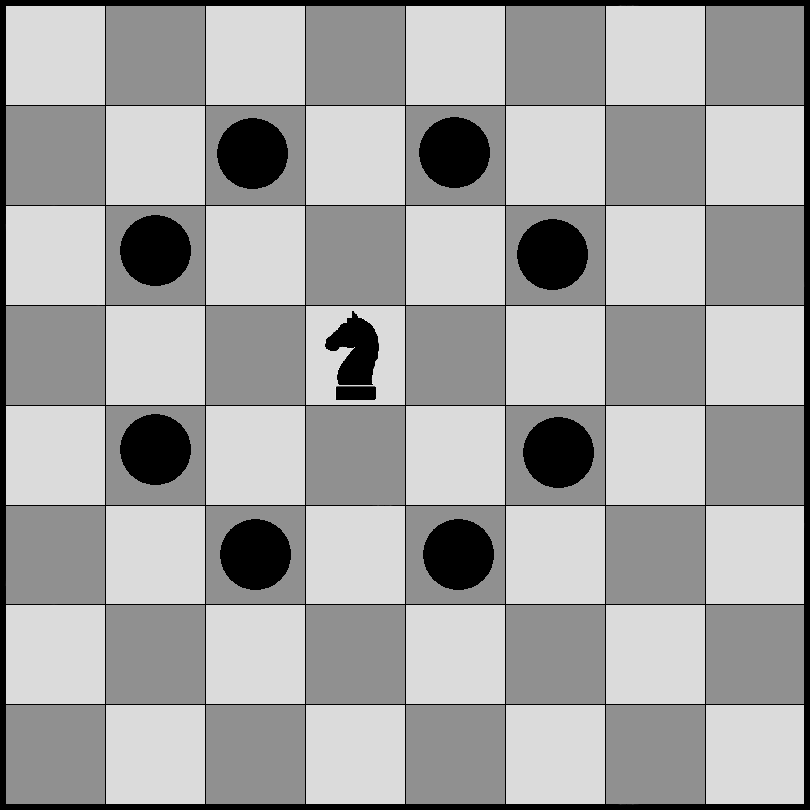
\includegraphics[scale=0.3]{imagenes/ej3/caballito.png}
 	\caption{Casillas que \emph{cubre} un caballo}
 	\label{caballito}	
   \end{center}
 \end{figure}


A continuaci\'on se pueden apreciar dos soluciones al problema de cubrir el tablero.

 \begin{figure}[h!]
   \begin{center}
 	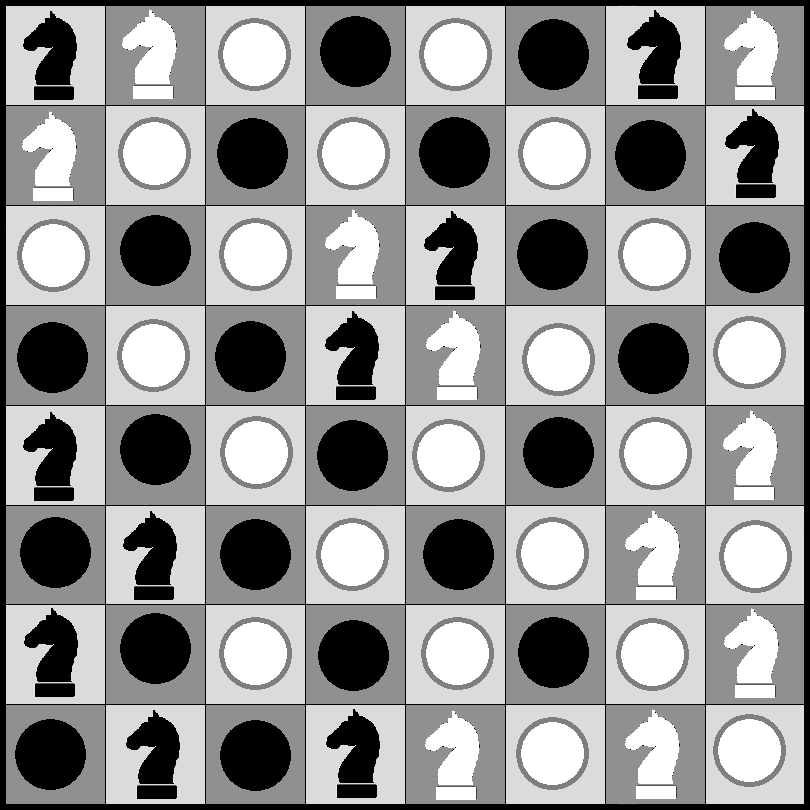
\includegraphics[scale=0.3]{imagenes/ej3/optimaCreo.png}
 	\caption{Soluci\'on 1}
% 	\label{optima_creo}	
   \end{center}
 \end{figure}
 
\newpage 
 
 
 \begin{figure}[h!]
   \begin{center}
 	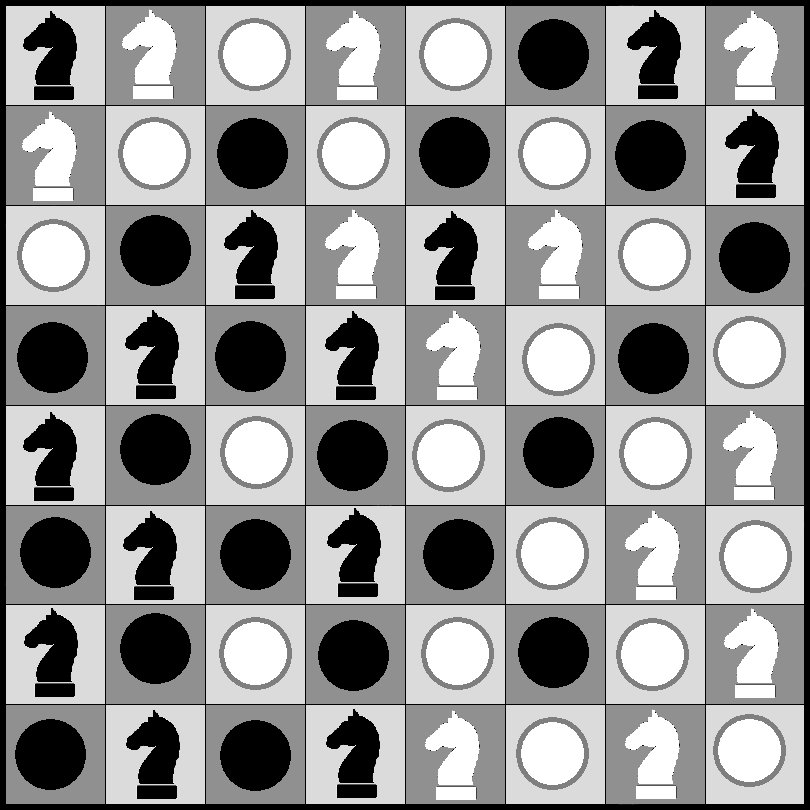
\includegraphics[scale=0.3]{imagenes/ej3/con5mas.png}
 	\caption{Soluci\'on 2}
 %	\label{con5mas}	
   \end{center}
 \end{figure}

En la soluci\'on 1 se necesitaron 20 caballos, en cambio en la dos 25; es decir 5 caballos m\'as. Por lo tanto podemos establecer que la soluci\'on 2 no es la \'optima y este caso no es lo que buscamos resolver. Por otro lado, la figura 1 \textcolor{red}{es \'optima? Despu\'es sabremos...}

\subsection{Resoluci\'on propuesta y justificaci\'on}

%re jodido esto amigooooo
%se ahcen todas las combinaciones y se va guardando la que tenga menor cantidad de caballos?

\subsection{An\'alisis de la complejidad}
\subsection{C\'odigo fuente}
\subsection{Experimentaci\'on}


% \section{Objetivos generales}

% El objetivo de este Trabajo Práctico es ...


% \section{Contexto}

% \begin{figure}
%   \begin{center}
% 	
\includegraphics[scale=0.66]{imagenes/logouba.jpg}
% 	\caption{Descripcion de la figura}
% 	\label{nombreparareferenciar}
%   \end{center}
% \end{figure}


% \paragraph{\textbf{Titulo del parrafo} } Bla bla bla bla.
% Esto se muestra en la figura~\ref{nombreparareferenciar}.




%Habra que insertar el enunciado???
% %\section{Enunciado y solucion} 
% %\input{enunciado}

% \section{Conclusiones y trabajo futuro}


\end{document}

